\section{Exercise 5}
\subsection*{5.1}
\begin{figure}[H]
	\centering
	\begin{subfigure}[b]{0.45\linewidth}
		\centering
		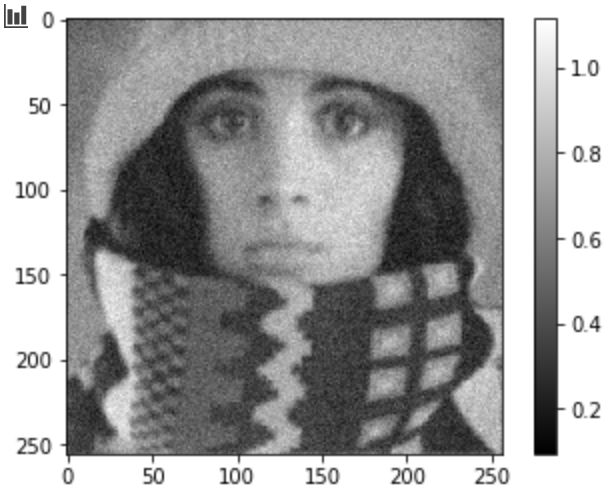
\includegraphics[width=\linewidth]{Materials/E5/gaus1std005}
		\caption{Gaussian kernel with $\sigma = 1$ and noise with standard deviation of $0.05$.}
	\end{subfigure}
	\hfill
	\begin{subfigure}[b]{0.45\linewidth}
		\centering
		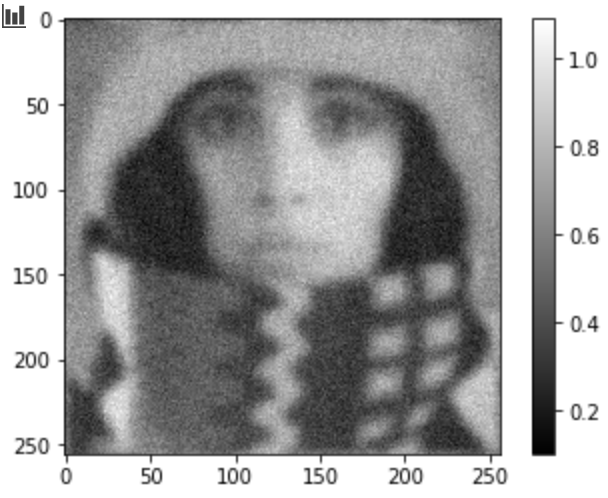
\includegraphics[width=\linewidth]{Materials/E5/gaus3std005}
		\caption{Gaussian kernel with $\sigma = 3$ and noise with standard deviation of $0.05$.}
	\end{subfigure}
	\\
	\begin{subfigure}[b]{0.45\linewidth}
		\centering
		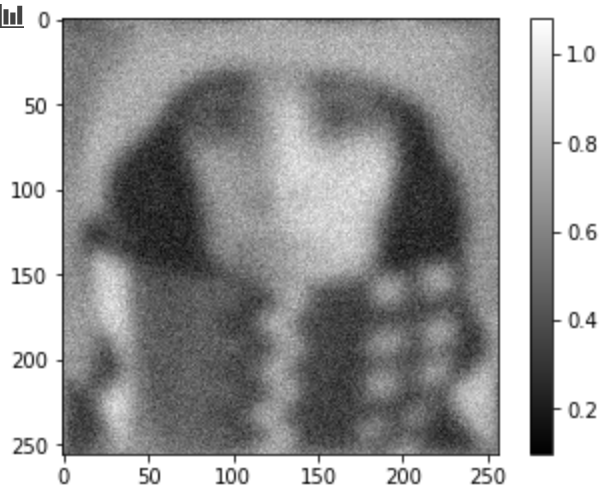
\includegraphics[width=\linewidth]{Materials/E5/gaus5std005}
		\caption{Gaussian kernel with $\sigma = 5$ and noise with standard deviation of $0.05$.}
	\end{subfigure}
	\hfill
	\begin{subfigure}[b]{0.45\linewidth}
		\centering
		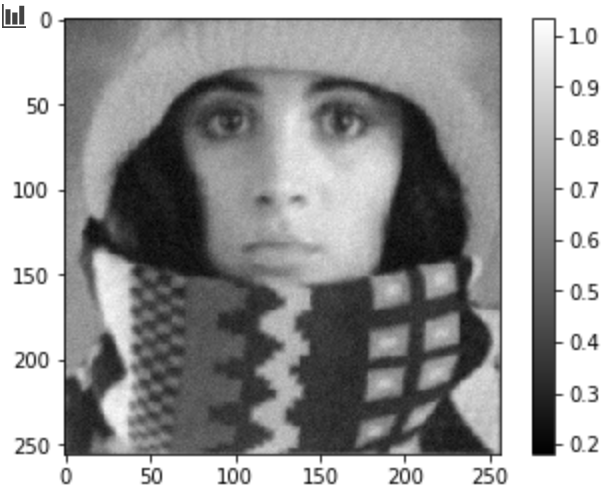
\includegraphics[width=\linewidth]{Materials/E5/gaus1std002}
		\caption{Gaussian kernel with $\sigma = 1$ and noise with standard deviation of $0.02$.}
	\end{subfigure}
	\\
	\begin{subfigure}[b]{0.45\linewidth}
		\centering
		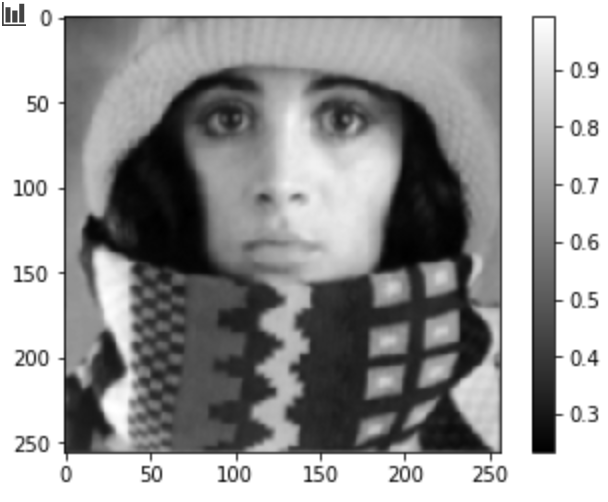
\includegraphics[width=\linewidth]{Materials/E5/gaus1std0001}
		\caption{Gaussian kernel with $\sigma = 1$ and noise with standard deviation of $0.001$.}
	\end{subfigure}
	\caption{Results of linear shift invariant degradation model with different noise and blurring factors.}
	\label{LSI}
\end{figure}
In \autoref{LSI} we see the results of the linear shift invariant degradation model. In the first three images the $\sigma$ values of the kernel is changing while the noise is kept constant, and in the last two images the $\sigma$ is kept constant while we turn down the noise levels. The realization of the noise is created by drawing as many samples with \textit{np.random.normal} as there are pixels in the image with a mean of 0. We control the strength of the noise by tuning the standard deviation. To make the noise visual we normalize the trui image so all values are between 0 and 1. We see the noise is quite significant when the standard deviation is around $0.05$, it is visible around $0.02$ and almost gone at around $0.001$. The code used for this exercise can be seen in \autoref{E51code}.
\begin{figure}[H]
	\centering
	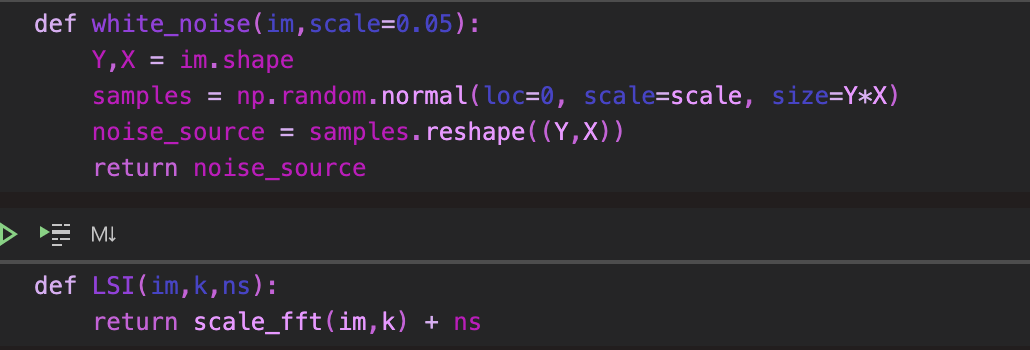
\includegraphics[width=0.8\linewidth]{Materials/E5/E51code}
	\caption{Code used for this exercise. \textit{scale\_fft} is a utility function which convolves an image and a kernel in frequency space.}
	\label{E51code}
\end{figure}

\subsection*{5.2}
\begin{figure}[H]
	\centering
	\begin{subfigure}[b]{0.45\linewidth}
		\centering
		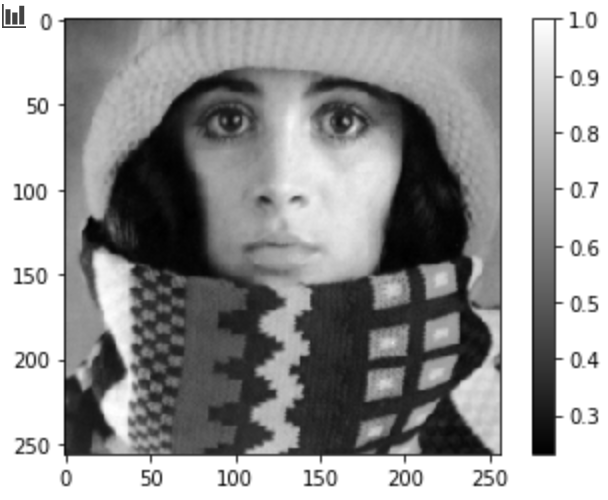
\includegraphics[width=\linewidth]{Materials/E5/dbn0}
		\caption{Gaussian kernel with $\sigma = 3$ and no noise.\\\hfill}
	\end{subfigure}
	\hfill
	\begin{subfigure}[b]{0.45\linewidth}
		\centering
		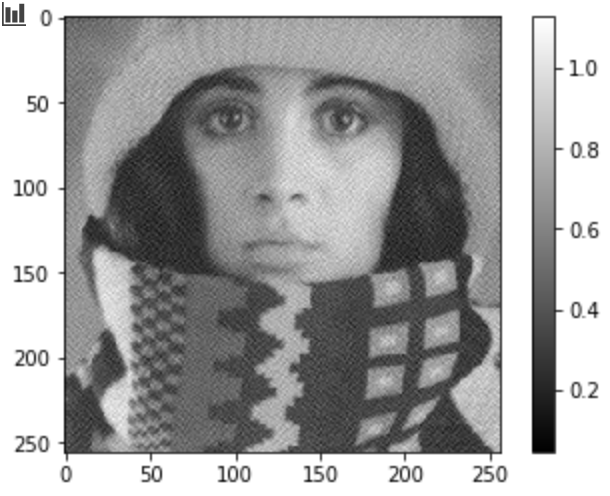
\includegraphics[width=\linewidth]{Materials/E5/dbn000000002}
		\caption{Gaussian kernel with $\sigma = 3$ and noise with standard deviation of $0.000000002$.}
	\end{subfigure}
	\\
	\begin{subfigure}[b]{0.45\linewidth}
		\centering
		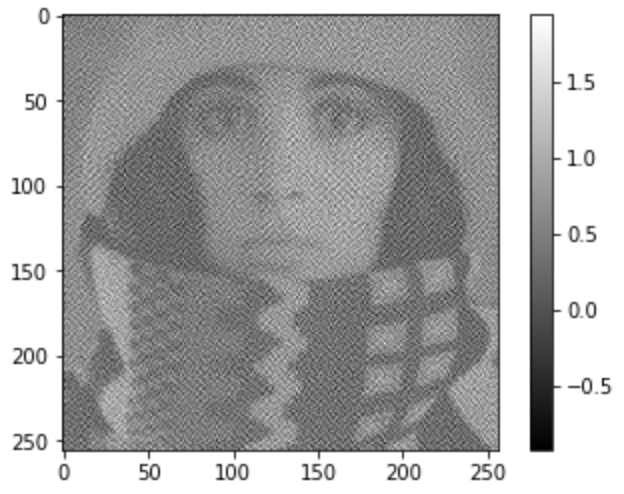
\includegraphics[width=\linewidth]{Materials/E5/dbn00000001}
		\caption{Gaussian kernel with $\sigma = 3$ and noise with standard deviation of $0.00000001$.}
	\end{subfigure}
	\hfill
	\begin{subfigure}[b]{0.45\linewidth}
		\centering
		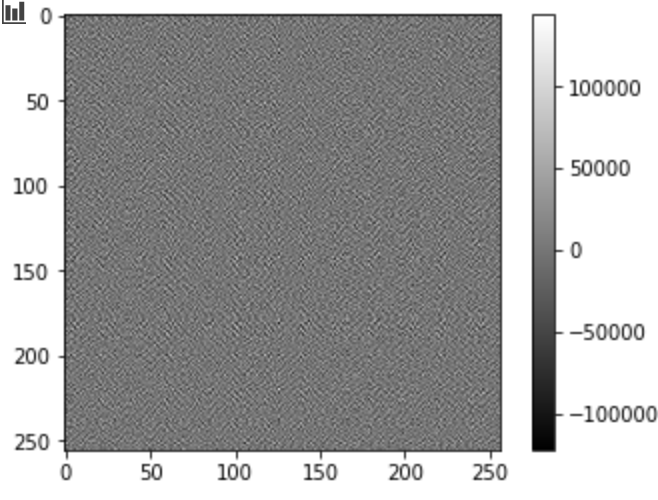
\includegraphics[width=\linewidth]{Materials/E5/dbn001}
		\caption{Gaussian kernel with $\sigma = 3$ and noise with standard deviation of $0.001$.}
	\end{subfigure}
	\caption{Results of direct inverse filtering with different strengths of noise.}
	\label{DirectInverse}
\end{figure}
In \autoref{DirectInverse} we see the results of applying direct inverse filtering on the LSI degraded image where we have blurred the image with a Gaussian kernel with $\sigma = 3$. We simply take the Fourier transform of the LSI degraded image and the psf and then divide the image with the psf. As we see, when there are no noise present the restoration results are very good, and all the blurring disappears. However, when we add just a tiny bit of noise it can be seen in the result. Already when we add noise with a standard deviation of $0.00000001$ the results becomes almost useless, and when we further increase the noise we simply get garbage. Thus we conclude that the direct inverse filtering approach works very well when there are no noise, but really quickly we get garbage if noise is present. In \autoref{E52code} we see the code used for this exercise.
\begin{figure}[H]
	\centering
	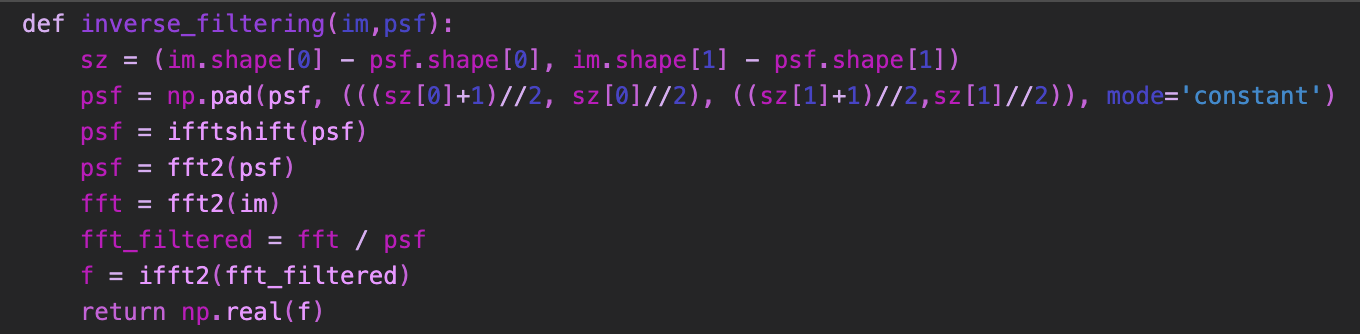
\includegraphics[width=\linewidth]{Materials/E5/E52code}
	\caption{Code used for this exercise.}
	\label{E52code}
\end{figure}

\subsection*{5.3}
\begin{figure}[H]
	\centering
	\begin{subfigure}[b]{0.45\linewidth}
		\centering
		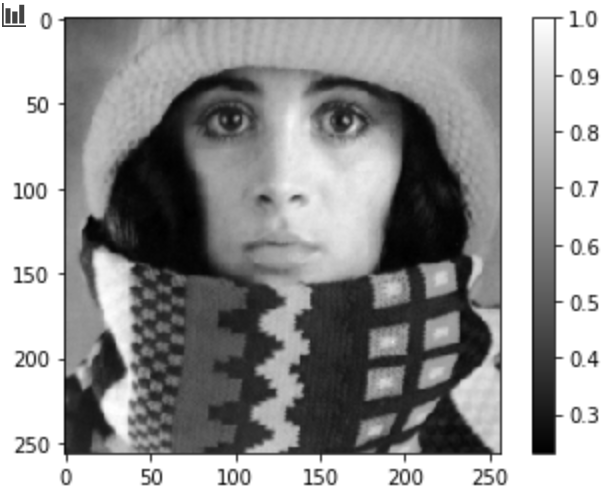
\includegraphics[width=\linewidth]{Materials/E5/w1}
		\caption{Gaussian kernel with $\sigma = 3$, no noise and $k = 0$.\\\hfill}
	\end{subfigure}
	\hfill
	\begin{subfigure}[b]{0.45\linewidth}
		\centering
		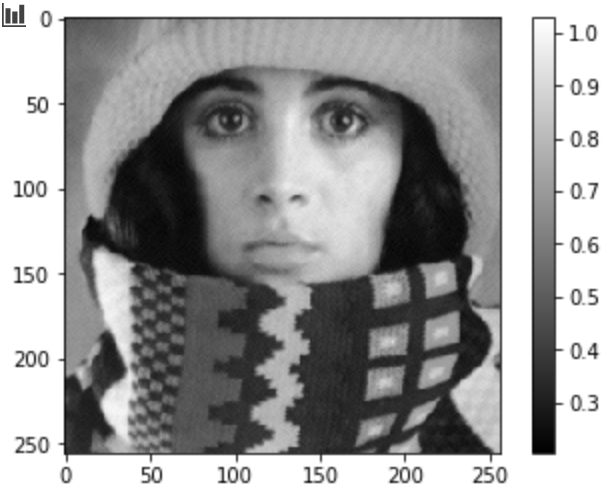
\includegraphics[width=\linewidth]{Materials/E5/w2}
		\caption{Gaussian kernel with $\sigma = 3$, noise with standard deviation of $0.000000002$ and $k = 0.000000000000001$.}
	\end{subfigure}
	\\
	\begin{subfigure}[b]{0.45\linewidth}
		\centering
		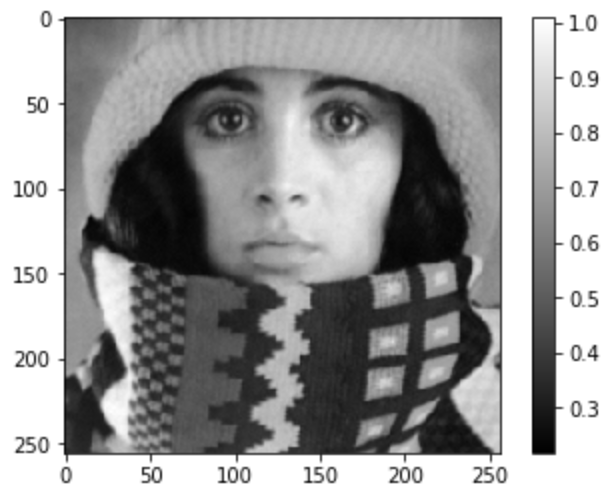
\includegraphics[width=\linewidth]{Materials/E5/w3}
		\caption{Gaussian kernel with $\sigma = 3$, noise with standard deviation of $0.00000001$ and $k = 0.0000000000005$.}
	\end{subfigure}
	\hfill
	\begin{subfigure}[b]{0.45\linewidth}
		\centering
		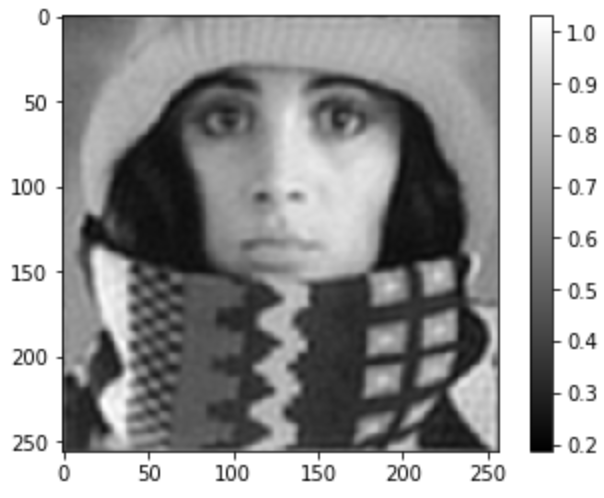
\includegraphics[width=\linewidth]{Materials/E5/w4}
		\caption{Gaussian kernel with $\sigma = 3$, noise with standard deviation of $0.001$ and $k = 0.0005$.}
	\end{subfigure}
	\caption{Results of Wiener filtering with different strengths of noise.}
	\label{wienercompare}
\end{figure}
In \autoref{wienercompare} we see the results of the Wiener filter on the same images as in the previous exercise. We here see a clear performance increase as the first 3 images are restored to perfection and the last is only slightly blurred still. In \autoref{wienerextreme} we see some examples of Wiener filtering on images with a little more extreme noise and blurring. In the first image we see an image almost completely gone in noise, and although the Weiener filter can not remove neither the noise or blurring completely, we still see a silhouette of the trui image with a clear scarf pattern, an indication of mouth and nose and blurred eye sockets. The second image is not completely gone in noise, but still heavily covered, and the result is a more clear image with both blurring and noise, but not disturbingly much noise. In additions to the features we could see in the previous image we can now clearly see the eyes, nostrils and eyebrows. In the last image the noise has been tuned down, but the blurring has been increased. The result is the most clear of the three, but still covered in both noise and blurring, but the restored image is clear.\\
During the experimentation with \textit{k} values, noise and blurring I note that to decrease the blurring we want a small \textit{k} value, whereas to remove noise, we want a high \textit{k} value. Because of this, a lot of the restored image has been a compromise between removing enough noise to see the underlying image, but also removing the blurring effect.\\
We see that the Wiener filter can to a high degree restore the image to a clear state where most features can be seen clearly if we apply low to medium noise, and can it can restore a fairly good silhouette of the image when the noise becomes high. Thus its abilities to restore images are good.\\
The code for this exercise can be seen in \autoref{E53code}. We here take the Fourier transform of the image and the psf and implement eq. 5.8-6 from Gonzales and Woods.

\begin{figure}[H]
	\centering
	\begin{subfigure}[b]{0.45\linewidth}
		\centering
		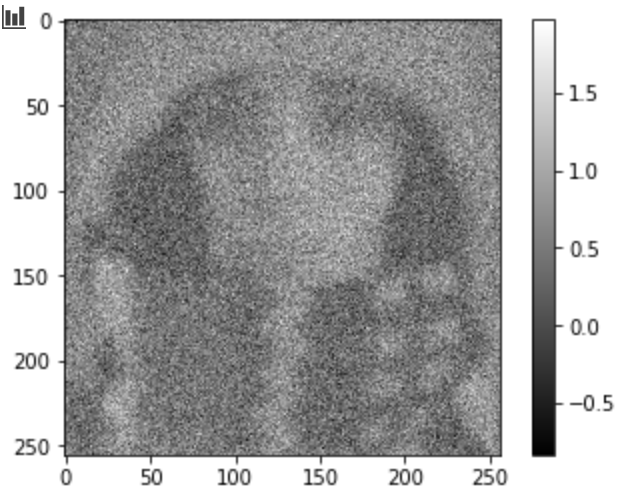
\includegraphics[width=\linewidth]{Materials/E5/w5before}
		\caption{LSI degraded image with Gaussian kernel with $\sigma = 3$ and noise with standard deviation of $0.3$ .}
	\end{subfigure}
	\hfill
	\begin{subfigure}[b]{0.45\linewidth}
		\centering
		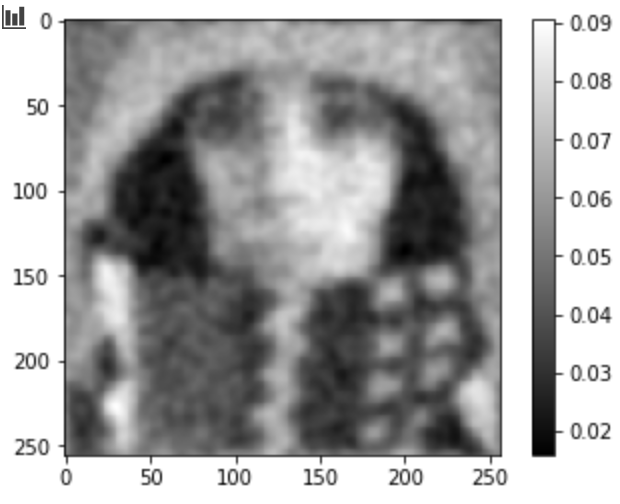
\includegraphics[width=\linewidth]{Materials/E5/w5after}
		\caption{Wiener result on LSI degraded image with Gaussian kernel with $\sigma = 3$, noise with standard deviation of $0.3$ and $k = 10$.}
	\end{subfigure}
	\\
	\begin{subfigure}[b]{0.45\linewidth}
		\centering
		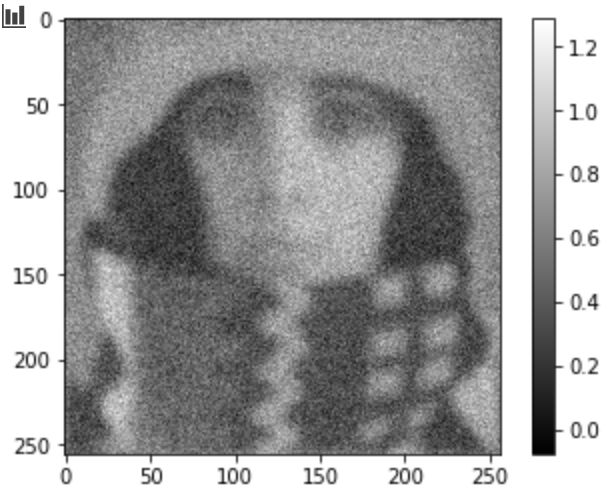
\includegraphics[width=\linewidth]{Materials/E5/w6before}
		\caption{LSI degraded image with Gaussian kernel with $\sigma = 3$ and noise with standard deviation of $0.1$.}
	\end{subfigure}
	\hfill
	\begin{subfigure}[b]{0.45\linewidth}
		\centering
		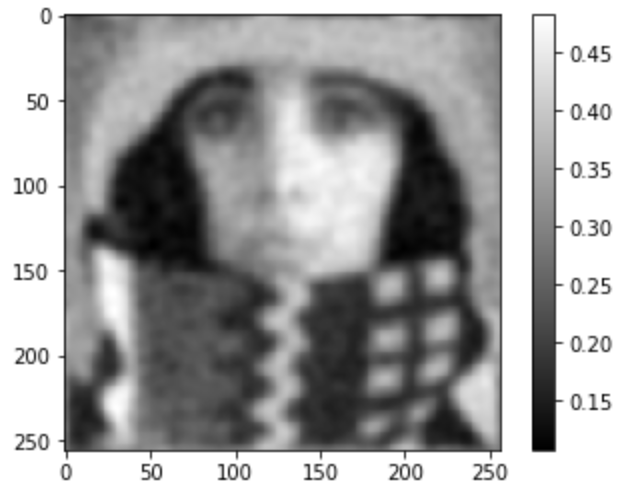
\includegraphics[width=\linewidth]{Materials/E5/w6after}
		\caption{Wiener result on LSI degraded image with Gaussian kernel with $\sigma = 3$, noise with standard deviation of $0.1$ and $k = 1$.}
	\end{subfigure}
	\\
	\begin{subfigure}[b]{0.45\linewidth}
		\centering
		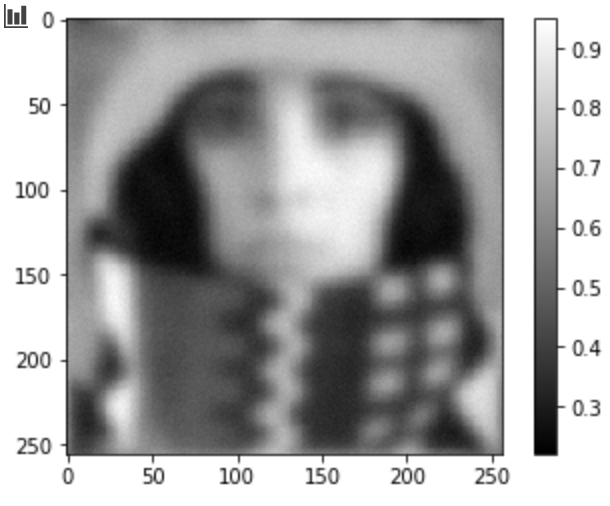
\includegraphics[width=\linewidth]{Materials/E5/w7before}
		\caption{LSI degraded image with Gaussian kernel with $\sigma = 5$ and noise with standard deviation of $0.01$.}
	\end{subfigure}
	\hfill
	\begin{subfigure}[b]{0.45\linewidth}
		\centering
		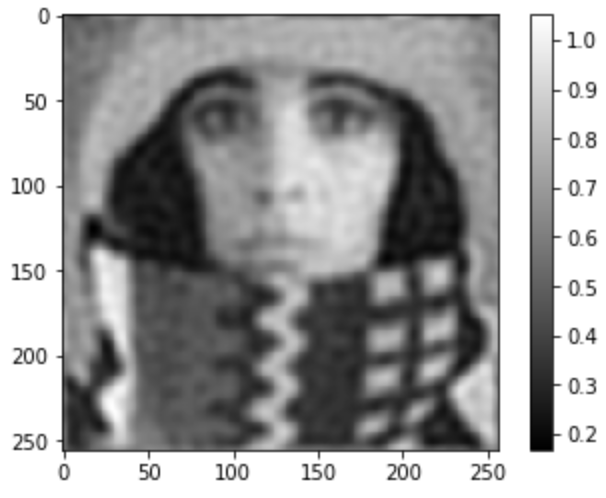
\includegraphics[width=\linewidth]{Materials/E5/w7after}
		\caption{Wiener result on LSI degraded image with Gaussian kernel with $\sigma = 5$, noise with standard deviation of $0.01$ and $k = 0.002$.}
	\end{subfigure}
	\caption{Results of Wiener filtering with different strengths of noise.}
	\label{wienerextreme}
\end{figure}

\begin{figure}[H]
	\centering
	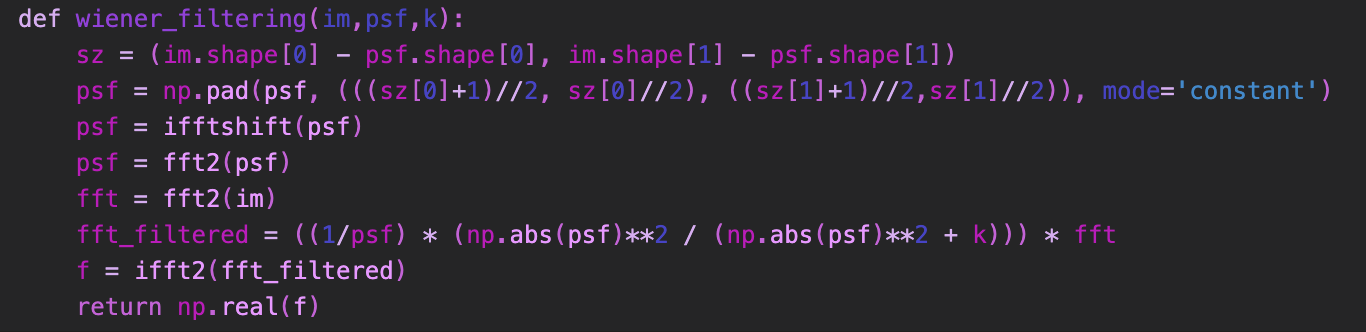
\includegraphics[width=\linewidth]{Materials/E5/E53code}
	\caption{Code used for this exercise.}
	\label{E53code}
\end{figure}